\chapter{Methodology}
\label{ch:methodology}

This chapter describes how LectureAssist is built: the overall system design and the
flow of data through it, the software components chosen and why, and the
implementation of each stage --- extraction, retrieval, the multi-agent generation
loop, the four question-generation pipelines whose prompts are given verbatim, the
two-agent answer cross-check, and the grading and adaptation layers.

\section{System Design}
\label{sec:meth-design}

LectureAssist is organised as a pipeline of specialist agents coordinated by an
orchestrator. The user supplies either a lecture video or a document (PDF, DOCX,
PPTX); the system converts it into a single grounded content representation, and
every downstream capability --- summary, quiz, chat, adaptive practice --- consumes
that representation rather than the raw media. The design is deliberately
staged so that each stage produces an artifact that can be inspected, cached and
re-used, which is what makes the expensive stages (OCR, transcription) survivable
on free-tier hardware.

\begin{figure}[h]
    \centering
    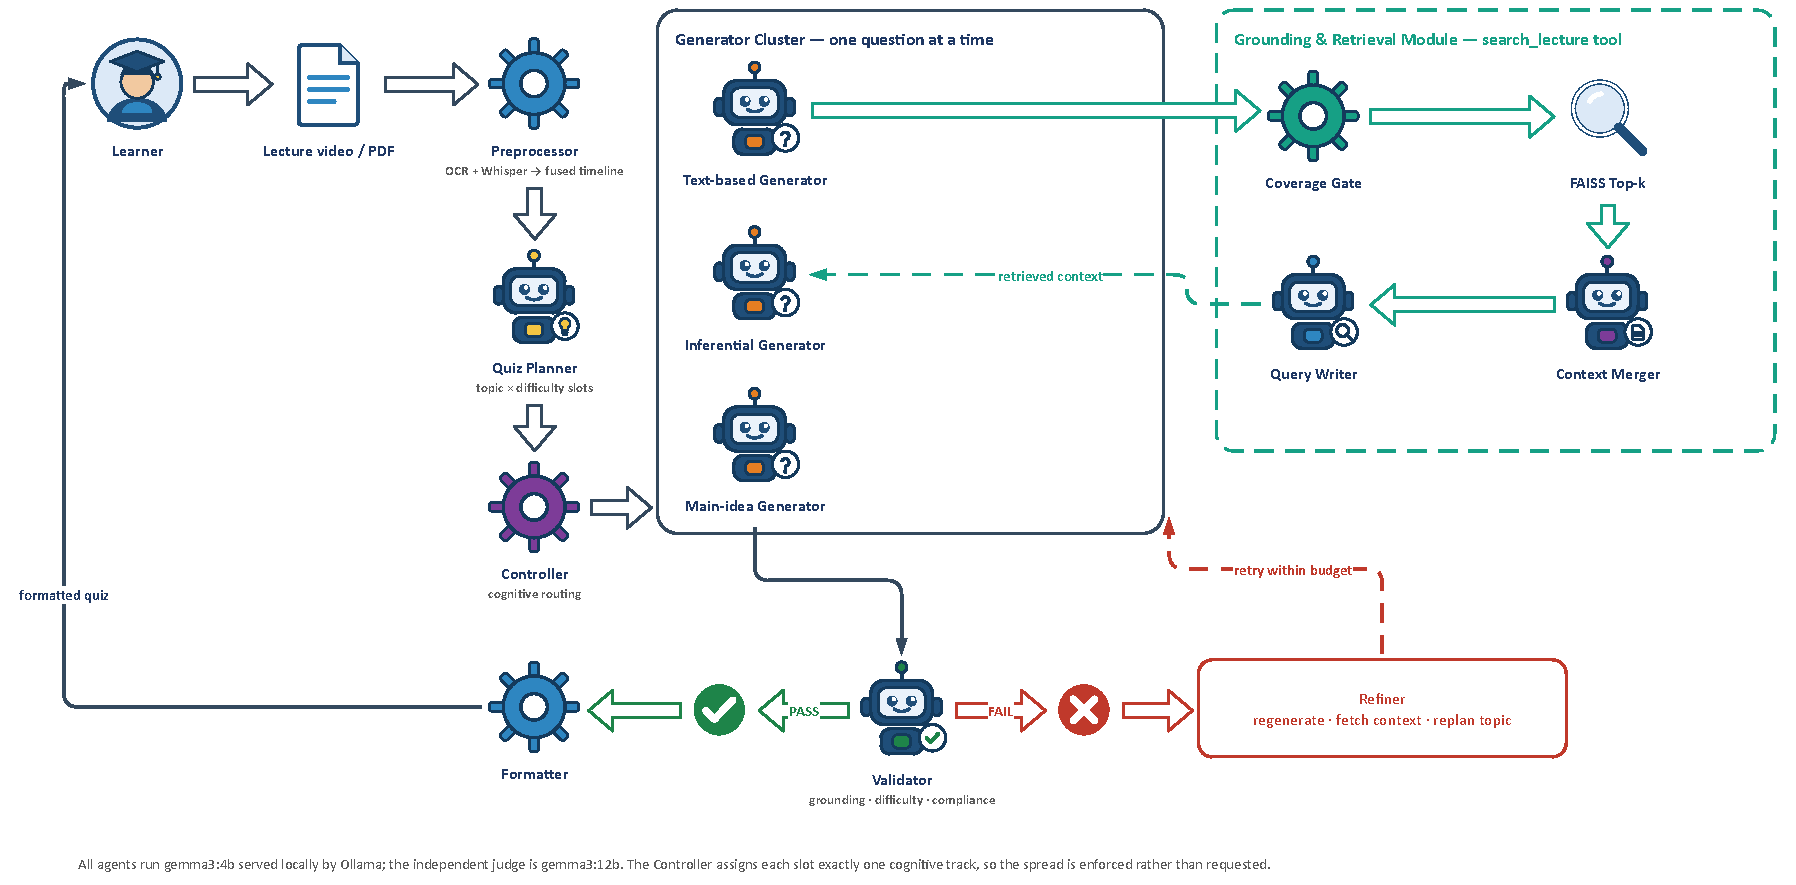
\includegraphics[width=\textwidth,height=30cm,keepaspectratio]{lectureassist-architecture-illustrated.pdf}
    \caption{System architecture of LectureAssist. The orchestrator coordinates
    specialist agents across ingestion, representation and generation: the
    Controller routes each slot to one of three cognitive tracks, the Validator
    accepts or rejects each drafted question, and a rejected question is
    diagnosed and returned to the Refiner rather than discarded. The dashed
    module on the right is the model-directed \texttt{search\_lecture}
    retrieval tool.}
    \label{fig:metho}
\end{figure}

\subsection{Data flow}
\label{sec:meth-flow}

The end-to-end flow is as follows.

\begin{enumerate}
  \item \textbf{Ingestion.} A video is sampled into frames and its audio track is
        demuxed; a document is parsed page by page.
  \item \textbf{Dual-channel extraction.} The visual channel goes to the
        \emph{Extractor} agent (scene-adaptive OCR); the audio channel goes to the
        \emph{Transcriber} agent (Faster-Whisper). Documents bypass both and go to
        the \emph{DocParser} agent.
  \item \textbf{Fusion.} OCR blocks and transcript segments are merged in
        timestamp order into a single unified lecture timeline, so that what the
        lecturer \emph{said} sits next to what they \emph{wrote} at the same moment.
  \item \textbf{Understanding.} The \emph{Summary} agent produces a structured
        summary; the \emph{RAG-Builder} agent chunks the content, embeds it and
        builds a vector index; the \emph{Hints} agent flags passages the lecturer
        marked as exam-relevant.
  \item \textbf{Generation.} The \emph{Quiz Planner} allocates questions across
        topics and difficulties; a \emph{Question Generator} drafts one question at
        a time; a \emph{Validator} accepts or rejects it and chooses a remediation
        action; a \emph{Refiner} applies it. This loop is the core of the system and
        is described in Section~\ref{sec:meth-agentic}.
  \item \textbf{Assessment and adaptation.} Answers are graded by a multi-tier
        grader; per-topic performance is written to a persistent profile, which the
        \emph{Adaptive Quiz} agent uses to bias the next quiz toward weak topics.
\end{enumerate}

\subsection{Scene-adaptive extraction}
\label{sec:meth-ocr}

A single OCR preprocessing recipe cannot handle a real lecture. White chalk on a
dark board is a low-contrast, inverted-polarity image; a projected slide in a lit
room is a bright, high-contrast one; a dark-theme slide deck looks superficially
like a blackboard but is destroyed by the inversion that a blackboard requires.
LectureAssist therefore \emph{classifies each sampled frame first} and preprocesses
it accordingly. Frames are routed by brightness and edge statistics into four
classes --- \texttt{slide}, \texttt{blackboard}, \texttt{whiteboard} and generic
\texttt{scene} (on-screen text) --- and each class gets its own contrast
enhancement, thresholding and, where appropriate, polarity inversion before being
passed to EasyOCR~\cite{easyocr}. Consecutive frames whose extracted text is more than $78\%$
similar are treated as the same board state and deduplicated, so that a slide left
on screen for two minutes contributes one block rather than sixty.

\subsection{Retrieval}
\label{sec:meth-rag}

Every generated artifact is grounded by retrieval-augmented
generation~\cite{lewis2020rag,gao2023ragsurvey}: the model is never asked to
recall the lecture from its weights, only to work from passages retrieved out of
the lecture itself.

The fused timeline is chunked and embedded with the Sentence-BERT
model~\cite{reimers2019sbert} \texttt{all-\allowbreak MiniLM-\allowbreak
L6-\allowbreak v2}~\cite{wang2020minilm}. The vectors are $L_2$-normalised and
indexed in FAISS~\cite{johnson2019faiss} with an inner-product index, so that
inner product equals cosine similarity (Eq.~\ref{eq:cosine}):
\begin{equation}
\label{eq:cosine}
\mathrm{sim}(q, c) \;=\;
  \frac{\mathbf{e}_q \cdot \mathbf{e}_c}
       {\lVert \mathbf{e}_q \rVert \, \lVert \mathbf{e}_c \rVert}
  \;=\; \hat{\mathbf{e}}_q \cdot \hat{\mathbf{e}}_c ,
  \qquad
  \hat{\mathbf{e}} = \frac{\mathbf{e}}{\lVert \mathbf{e} \rVert},
\end{equation}
where $\mathbf{e}_q, \mathbf{e}_c \in \mathbb{R}^{384}$ are the embeddings of the
query and of a candidate chunk. Because every vector is $L_2$-normalised before
insertion, the denominator is unity and a plain inner-product search returns exactly
the cosine ranking, which is why no separate normalisation step is needed at query
time. Retrieval returns the top
$k = 5$ chunks together with their timestamps, which is what allows both the chat
interface and a generated question to be traced back to the moment in the lecture
they came from. Crucially, retrieval is exposed to the generator agent as a
\emph{tool} (\texttt{search\_lecture}) rather than being applied unconditionally:
the agent decides for itself whether it needs more evidence.

\section{Hardware and/or Software Components}
\label{sec:meth-components}

The system is written in Python and served as a Flask~\cite{flask} API, with a single-page
HTML/JavaScript front end that talks to it over an ngrok~\cite{ngrok} tunnel; this split lets the
heavy models run on a Colab~\cite{colab} GPU while the interface runs in the student's own
browser. Table~\ref{tab:tools} lists the components, the alternatives considered,
and the reason for each choice. The overriding constraint throughout was that
\emph{nothing may require a paid API key}, since the target users are precisely
those for whom a per-token bill is prohibitive.

\begin{table}[H]
\centering
\caption{Software components, alternatives, and selection rationale.}
\label{tab:tools}
\footnotesize
\begin{tabular}{|p{2.6cm}|p{3.0cm}|p{3.2cm}|p{4.4cm}|}
\hline
\textbf{Tool} & \textbf{Function} & \textbf{Other similar tools} & \textbf{Why selected} \\
\hline
Gemma~3 (4B / 12B) & Generation, summarisation, grading, judging &
GPT-4, Claude, Llama~3, Mistral &
Open weights, runs locally, no API key; two sizes let the cheap model generate and
the strong model judge. \\
\hline
Ollama & Local LLM serving &
llama.cpp, vLLM, HF Transformers &
One-line model pull, automatic GPU offload, OpenAI-style local HTTP API; vLLM needs
more VRAM than a free T4 has. \\
\hline
Faster-Whisper (\texttt{small}) & Speech-to-text &
OpenAI Whisper API, Vosk, wav2vec2 &
Same accuracy as reference Whisper at a fraction of the memory; runs offline. The
API version is paid and cloud-bound. \\
\hline
EasyOCR (en, bn) & Board and slide text extraction &
Tesseract, PaddleOCR, Google Vision &
Deep-learning based, far better on handwriting than Tesseract; native Bengali
support matters for local lectures; Google Vision is a paid cloud API. \\
\hline
Sentence-Transformers \texttt{all-MiniLM-L6-v2} & Embeddings for RAG and for evaluation metrics &
OpenAI \texttt{text-embedding-3}, BGE, E5 &
$384$-dim, small and fast enough to co-exist with the LLM on one GPU; strong
quality-per-byte; local. \\
\hline
FAISS & Vector index &
Chroma, Pinecone, pgvector &
In-process, no server, no network; exact inner-product search is more than
sufficient at lecture scale. \\
\hline
PyMuPDF~\cite{pymupdf} & PDF/DOCX/PPTX parsing &
pdfplumber, PyPDF2 &
Fastest reliable text-layer extraction; preserves page structure used for
per-page source attribution. \\
\hline
Flask + ngrok & Backend API and public tunnel &
FastAPI, Gradio, Streamlit &
Minimal surface for a JSON API; ngrok exposes the Colab GPU to a browser UI running
on the student's own machine. \\
\hline
SymPy & Building the verified answer key for calibration &
Hand-computed answers, WolframAlpha &
Answers are \emph{machine-computed}, not hand-typed, so the calibration set cannot
inherit a human arithmetic error. \\
\hline
Google Colab (T4) + Drive & Compute and persistence &
Local GPU, RunPod, AWS &
Free tier is the realistic deployment target; Drive persistence lets a run survive
a runtime disconnect. \\
\hline
\end{tabular}
\end{table}

\section{Hardware and/or Software Implementation}
\label{sec:meth-impl}

\subsection{The agentic question-generation loop}
\label{sec:meth-agentic}

The agentic Question Generator produces \emph{one question at a time} through a
multi-stage loop. The design decision that distinguishes it from a
generate-then-filter pipeline is that the validator does not merely reject a bad
question --- it \emph{diagnoses} it and chooses how the next attempt should differ.
The stages are:

\begin{enumerate}
  \item \textbf{Plan.} The Quiz Planner reads the lecture summary and distributes
        the requested questions across the topics that are actually present, each
        with a target difficulty, yielding a list of (topic, difficulty) slots.
  \item \textbf{Retrieve.} Before drafting a slot, the generator inspects the content
        it holds and decides for itself whether it has enough material on that topic.
        If not, it issues its own retrieval query through the
        \texttt{search\_lecture} tool to pull more context. This is genuine tool use:
        the decision to retrieve is the model's, not a fixed step in the pipeline.
  \item \textbf{Generate.} It drafts exactly one question under a grounding rule ---
        the question must be answerable using only the supplied content --- rotating
        a question strategy on each attempt (concept-check, scenario,
        compare-and-justify) so that a retry is not merely a resample of the same
        prompt.
  \item \textbf{Validate.} A separate call checks the draft on three axes ---
        difficulty match, grounding, and instruction compliance --- and returns
        \texttt{PASS} or \texttt{FAIL} together with a remediation \texttt{action}.
  \item \textbf{Retry (loop back).} On \texttt{FAIL} the loop repeats within a retry
        budget, and the validator's chosen action decides the fix:
        \texttt{regenerate} (rewrite, with the failure reason fed back into the
        prompt), \texttt{fetch\_context} (retrieve more evidence first, then retry),
        or \texttt{replan\_topic} (abandon a topic that is not really in the lecture
        and swap to one that is).
  \item \textbf{Override.} If the retry budget is exhausted, the best attempt so far
        is kept and explicitly \emph{labelled} as an override. It is never silently
        recorded as a clean pass --- otherwise the pipeline's own accept rate would
        be a fiction.
\end{enumerate}

\begin{figure}[H]
\centering
\begin{tikzpicture}[x=1cm, y=1cm]

  % --- main chain -----------------------------------------------------------
  \node[laproc, text width=20mm] (plan) at (0,0)
       {Planner\\{\normalfont\scriptsize topic $+$ difficulty slots}};
  \node[lallm, text width=22mm]  (gen)  at (3.9,0)
       {Generator\\{\normalfont\scriptsize drafts ONE question}};
  \node[laval, text width=24mm]  (val)  at (8.1,0)
       {Validator\\{\normalfont\scriptsize grounding, difficulty, compliance}};
  \node[laout, text width=18mm]  (acc)  at (12.1,0)
       {Accept\\{\normalfont\scriptsize next slot}};

  % --- retrieval tool -------------------------------------------------------
  \node[latool, text width=34mm] (tool) at (3.9,2.15)
       {\texttt{search\_lecture}\\{\normalfont\scriptsize model-directed retrieval}};

  % --- remediation ----------------------------------------------------------
  \node[lallm, text width=53mm] (ref) at (8.3,-2.85)
       {Refiner\\{\normalfont\small the validator picks the fix}\\[1pt]
        {\normalfont\scriptsize \texttt{regenerate} $\;\cdot\;$
         \texttt{fetch\_context} $\;\cdot\;$ \texttt{replan\_topic}}};

  % --- edges ----------------------------------------------------------------
  \draw[laarr]  (plan) -- (gen);
  \draw[laarr]  (gen)  -- (val);
  \draw[laarrg] (val)  -- (acc) node[lalbl, midway, above]{PASS};
  \draw[laarrc] (tool) -- (gen)
        node[lalbl, midway, right]{evidence};
  \draw[laloop] (val.south) -- (ref.north)
        node[lalbl, midway, right]{FAIL};
  \draw[laloop] (ref.west) -| (gen.south)
        node[lalbl, pos=0.28, below]{retry $\leq 3$};
  \draw[laarr, draw=LAslate] (ref.south) -- ++(0,-0.75) -| (acc.south)
        node[lalbl, pos=0.30, below]
        {budget exhausted: keep best attempt, mark as override};

\end{tikzpicture}
\caption{The agentic question-generation loop. Questions are produced one at a time
and must pass validation before the next slot begins. The dashed edge is genuine
tool use: the generator decides for itself whether it has enough grounding and issues
its own retrieval query if not. On \texttt{FAIL} the validator does not merely
reject --- it selects the remediation, and only \texttt{regenerate} returns to the
generator directly, while \texttt{fetch\_context} and \texttt{replan\_topic} require
work outside the model first. When the retry budget is exhausted the best attempt is
kept but is explicitly labelled an override, so that a failure is never recorded as a
clean pass.}
\label{fig:agentic-loop}
\end{figure}

\subsection{Agent contracts and failure behaviour}
\label{sec:meth-contracts}

Every agent in the system inherits from a common base class and honours the same
four-stage contract: \texttt{should\_run}, which lets an agent decline work it
has no input for; \texttt{plan}, which records what it intends to do;
\texttt{execute}, which performs it; and \texttt{validate}, which checks its own
output before the orchestrator accepts it. The contract matters more than any
individual agent, because it is what makes the pipeline degrade rather than
fail: an agent that raises is caught by the orchestrator, its failure is written
to the agent log with the reason, and the remaining agents continue on whatever
context exists. A lecture whose audio track is unreadable still produces a
summary from board text alone.

Table~\ref{tab:agents} lists the agents, what each consumes and produces, and
what happens when it cannot do its job.

\begin{table}[H]
\centering
\caption{Agent contracts. Every agent validates its own output; the orchestrator
isolates failures so that one agent cannot abort the run.}
\label{tab:agents}
\footnotesize
\setlength{\tabcolsep}{4pt}
\begin{tabular}{|p{2.5cm}|p{3.1cm}|p{3.1cm}|p{4.0cm}|}
\hline
\textbf{Agent} & \textbf{Consumes} & \textbf{Produces} & \textbf{On failure} \\
\hline
Extractor & Video frames & Board and slide text, timestamped &
Run continues on audio alone \\
\hline
Transcriber & Audio track & Transcript segments with timestamps &
Run continues on board text alone \\
\hline
DocParser & PDF, DOCX, PPTX & Structured document text &
Run aborts; there is no other source \\
\hline
Summarizer & Fused timeline or document text & Structured summary &
Validated for length and refusal patterns, then retried \\
\hline
RAGBuilder & Summary and fused timeline & FAISS index over chunks &
Generation falls back to the summary without retrieval \\
\hline
Hints & Summary and timeline & Ranked exam-focus topics &
Planner falls back to summary topics \\
\hline
QuizPlanner & Summary, weak-topic profile & (topic, difficulty) slots &
Falls back to an even spread over summary topics \\
\hline
Quiz generator (Easy / Medium / Hard) & One slot, retrieved context &
One draft question & Retried under the loop of
Section~\ref{sec:meth-agentic} \\
\hline
QuizValidator & Draft question, accepted set & PASS/FAIL plus a remediation
action & A failed parse is treated as FAIL, never as PASS \\
\hline
QuizRefiner & Failed draft and its reason & Revised draft &
Loop falls back to plain regeneration \\
\hline
Answer generator & Question without the marked key & Independently derived
answer & Item is flagged unverified, not dropped \\
\hline
\end{tabular}
\end{table}

Two of these entries carry the project's central design commitments. The
validator treats an unparseable response as \texttt{FAIL} rather than
\texttt{PASS}, so a malformed reply can never inflate the acceptance rate; and
the answer generator's disagreement flags an item rather than deleting it, so
that the disagreement rate remains measurable instead of being silently
engineered away.

\subsection{Reproducibility and experimental control}
\label{sec:meth-repro}

Because the evaluation in Chapter~\ref{ch:results} compares two pipelines, the
things held constant between them matter as much as the thing varied. This
subsection records them.

\paragraph{Models are pinned, not chosen at run time.} The generator is
\texttt{gemma3:4b} and the primary model, used for summarisation, judging and
grading, is \texttt{gemma3:12b}; both are open-weight and served locally through
Ollama. The generator is \emph{pinned}: when it returns unusable structured
output the system retries the same model with a stricter instruction rather than
escalating to the larger one. Escalation would have been the better engineering
choice for output reliability, and it was deliberately rejected, because a
pipeline that silently falls back to a $12$B model when the $4$B model struggles
would no longer be measuring what it claims to measure. Every question in
Chapter~\ref{ch:results} was written by the model the chapter names.

\paragraph{Decoding parameters.} All calls use temperature $0.2$, a context
window of $16{,}384$ tokens, and an output ceiling of $8{,}192$ tokens. The low
temperature reflects the task: structured assessment items with a single defensible
key, not creative text. The output ceiling is a correctness requirement rather
than a tuning choice --- without it the server truncates generation at a few
hundred tokens, which silently cuts structured output mid-object and presents as
the generator having produced nothing.

\paragraph{Thresholds are fixed in advance.} The uniqueness check rejects a draft
whose similarity to any already-accepted question exceeds $0.85$; the retry
budget is three attempts per slot; frame de-duplication during extraction
suppresses consecutive frames above $0.97$ similarity; and short-answer grading
accepts a fuzzy match above $0.80$. These values were set before the evaluation
run and were not adjusted after seeing results.

\paragraph{What is \emph{not} controlled, and why it matters.} Generation is
sampled rather than greedy, and no random seed is fixed, so the run is not
bit-for-bit reproducible: repeating it produces a different question set with
similar statistics. This is a real limitation for exact replication and is
stated rather than hidden. It is mitigated by sample size, $200$ questions per
pipeline, and by the fact that the reported differences are consistent across
three difficulty strata rather than resting on a single aggregate. Fixing a seed
is a cheap improvement and is listed among the further work in
Section~\ref{sec:concl-future}.

\paragraph{The artifact trail.} Each run writes the generated questions, the
per-question validator verdicts with attempt counts and timings, and the full
agent decision log. Measurement is performed offline on those artifacts rather
than inside the generating session, so that scoring cannot influence generation
and so that a scoring change can be re-applied to an existing run without
regenerating it. The labelling correction disclosed in
Section~\ref{sec:res-native} is the one place where this separation proved
insufficient, and it is the reason a confirming re-run is the first item of
further work.

\subsection{The four generation pipelines}
\label{sec:meth-pipelines}

To isolate the contribution of the agentic machinery, the same content is used to
generate questions through four pipelines that differ \emph{only} in how the model
is asked:

\begin{itemize}
  \item \textbf{Agentic} --- the Plan $\rightarrow$ Retrieve $\rightarrow$ Generate
        $\rightarrow$ Validate $\rightarrow$ Retry loop of
        Section~\ref{sec:meth-agentic}.
  \item \textbf{Non-agentic (plain)} --- a single LLM call that emits the questions
        directly: no planning, no retrieval, no validation, no retry.
  \item \textbf{Chain-of-thought (CoT)} --- a single call in which the model must
        reason step by step to \emph{derive} each answer before committing to it,
        and record that reasoning.
  \item \textbf{Program-of-thought (PoT)} --- a single call in which the model must
        derive each answer through an explicit, ordered sequence of computation steps
        (define, substitute, simplify, evaluate) and mark the option equal to the
        final computed value.
\end{itemize}

CoT and PoT are both \emph{single-shot and non-agentic}: one LLM call, no
planning, retrieval, validation or retry. The only thing that separates them from the
plain baseline is the wording of the prompt. They emit the same JSON schema as the
plain generator, plus one extra field (\texttt{reasoning} or \texttt{computation})
that is retained for inspection but ignored by the downstream judge and Answer
Generator, so all four pipelines feed into an identical scoring path and are
directly comparable. The two prompts are reproduced verbatim below, since the
prompt \emph{is} the method.

Placeholders in square brackets are substituted at call time: \texttt{[N]} is the
requested question count, \texttt{[DIFF]} the target difficulty band (that line is
omitted entirely when no band is requested), and \texttt{[CONTENT]} and
\texttt{[SUMMARY]} the retrieved lecture text and its summary, truncated to $8000$
and $1500$ characters respectively. Line breaks are those of the prompt as sent;
where a line is too long for the page it wraps with a $\hookrightarrow$ marker.

\begin{lstlisting}[style=prompt,caption={Chain-of-thought generation prompt, as
sent to the generator. The reasoning field is recorded for inspection and is
ignored by the judge and the Answer Generator.},label={lst:cot}]
Generate [N] high-quality MCQ from this lecture content.
Difficulty focus: [DIFF]
Use CHAIN-OF-THOUGHT: for EACH question, think step by step to work out the correct answer BEFORE choosing it, and record that step-by-step reasoning. The option you mark correct MUST be exactly the answer your reasoning reaches, and each distractor must be wrong for a stateable reason.
STRICT JSON: {"questions":[{"question","options":{"A","B","C","D"},"reasoning","correct_answer","explanation","topic","difficulty","bloom_level","source_timestamp","source_type"}]}
'reasoning' = your step-by-step derivation of the correct option.

CONTENT:
[CONTENT]

SUMMARY:
[SUMMARY]
\end{lstlisting}

% Kept whole on one page: a prompt split across a page break is hard to read as
% a single artifact, and these two are meant to be compared line for line.
\newpage
\begin{lstlisting}[style=prompt,caption={Program-of-thought generation prompt.
Identical to Prompt~\ref{lst:cot} except for the reasoning instruction and the
name of the recorded field, so the two differ only in how the answer is required
to be derived.},label={lst:pot}]
Generate [N] high-quality MCQ from this lecture content.
Difficulty focus: [DIFF]
Use PROGRAM-OF-THOUGHT: for EACH question, derive the answer through an explicit ordered sequence of computation/derivation steps (like a short program: define, substitute, simplify, evaluate), record those steps, and only then mark the option that EQUALS the final computed result. The marked correct option MUST equal the endpoint of your computation.
STRICT JSON: {"questions":[{"question","options":{"A","B","C","D"},"computation","correct_answer","explanation","topic","difficulty","bloom_level","source_timestamp","source_type"}]}
'computation' = your ordered derivation steps ending at the correct value.

CONTENT:
[CONTENT]

SUMMARY:
[SUMMARY]
\end{lstlisting}

% \subsection{Controlling for confounds}
% \label{sec:meth-controls}

% Two implementation details are needed for the comparison to be fair, and both were
% bugs before they were features.

% \paragraph{Model pinning.} The generator is pinned to \texttt{gemma3:4b}. The
% original implementation silently escalated to the $12$B model whenever the $4$B
% returned malformed JSON, which would have made the claim ``these questions were
% written by the $4$B'' false for exactly the hardest questions --- the ones where the
% $4$B struggles. Pinning costs some yield and is required for an honest study.

% \paragraph{Content coverage.} A generator that only ever reads the first $8{,}000$
% characters of a $92{,}000$-character chapter can only ever ask about the first few
% pages, and will necessarily repeat itself. Each baseline therefore reads through a
% \emph{sliding window} over the document, and --- critically --- all three baselines
% use the same batch size, so they receive the same number of windows and see the same
% share of the chapter. Otherwise a pipeline that happened to use a smaller batch
% would read more of the document, and any difference in its questions would be
% confounded by content coverage rather than caused by the prompt. Likewise, the
% lecture summary that the planner uses to pick topics is produced by \emph{map-reduce}
% summarisation over the whole document rather than by truncating it, so the planner
% can propose topics from any part of the chapter.

\subsection{Answer correctness: two agents that must agree}
\label{sec:meth-answer}

A question can be well written and still mark the wrong option. Question generation
and answer generation are therefore treated as \emph{two distinct agents}, and their
answers are cross-checked. Correctness is measured three complementary ways:

\begin{itemize}
  \item \textbf{Independent re-solve (Answer Generator agent).} The larger model is
        given the stem and the options \emph{with the marked answer removed}, and
        solves the question from scratch. Its choice is compared with the Question
        Generator's marked answer; the agreement rate is the
        \emph{independent-match rate}. The solver never sees what it is supposed to
        agree with.
  \item \textbf{Judge-verify.} While scoring quality, the judge is additionally
        asked whether the marked answer is actually correct given the content,
        yielding the \emph{judge-verified-correct rate}. This is free --- it rides
        along on a call that was already being made.
  \item \textbf{Calibration on a known-answer set.} The generated questions have no
        ground-truth key, so neither of the above is an absolute measure of
        correctness --- if generator and solver share a misconception, they agree
        and are both wrong. To bound this, both models independently solve a set of
        MCQ whose answers \emph{are} known, and their accuracy on it calibrates how
        much the agreement rate above is worth. The calibration set is stratified
        into \emph{computational} items, whose answers are computed with
        SymPy~\cite{sympy} rather than typed by hand, and \emph{conceptual} items
        drawn from the chapter's definitions and theorems. This is reported
        separately and is explicitly \emph{not} a score on the generated questions.
\end{itemize}

The calibration set is used for evaluation only. It is never placed on the
generation path, since a generator that had seen the answer key would be scored on
questions it had effectively been given, and the resulting numbers would be
contaminated.

\subsection{System snapshot}
\label{sec:meth-snapshot}

Figures~\ref{fig:ui-workspace} and~\ref{fig:ui-quiz} show the deployed system in
use. They are included because the agentic loop described in
Section~\ref{sec:meth-agentic} is not only an internal mechanism: it is surfaced
directly to the user, and one of the design commitments of this project is that a
student should be able to see how a question was produced rather than being handed
an opaque result.

\begin{figure}[H]
\centering
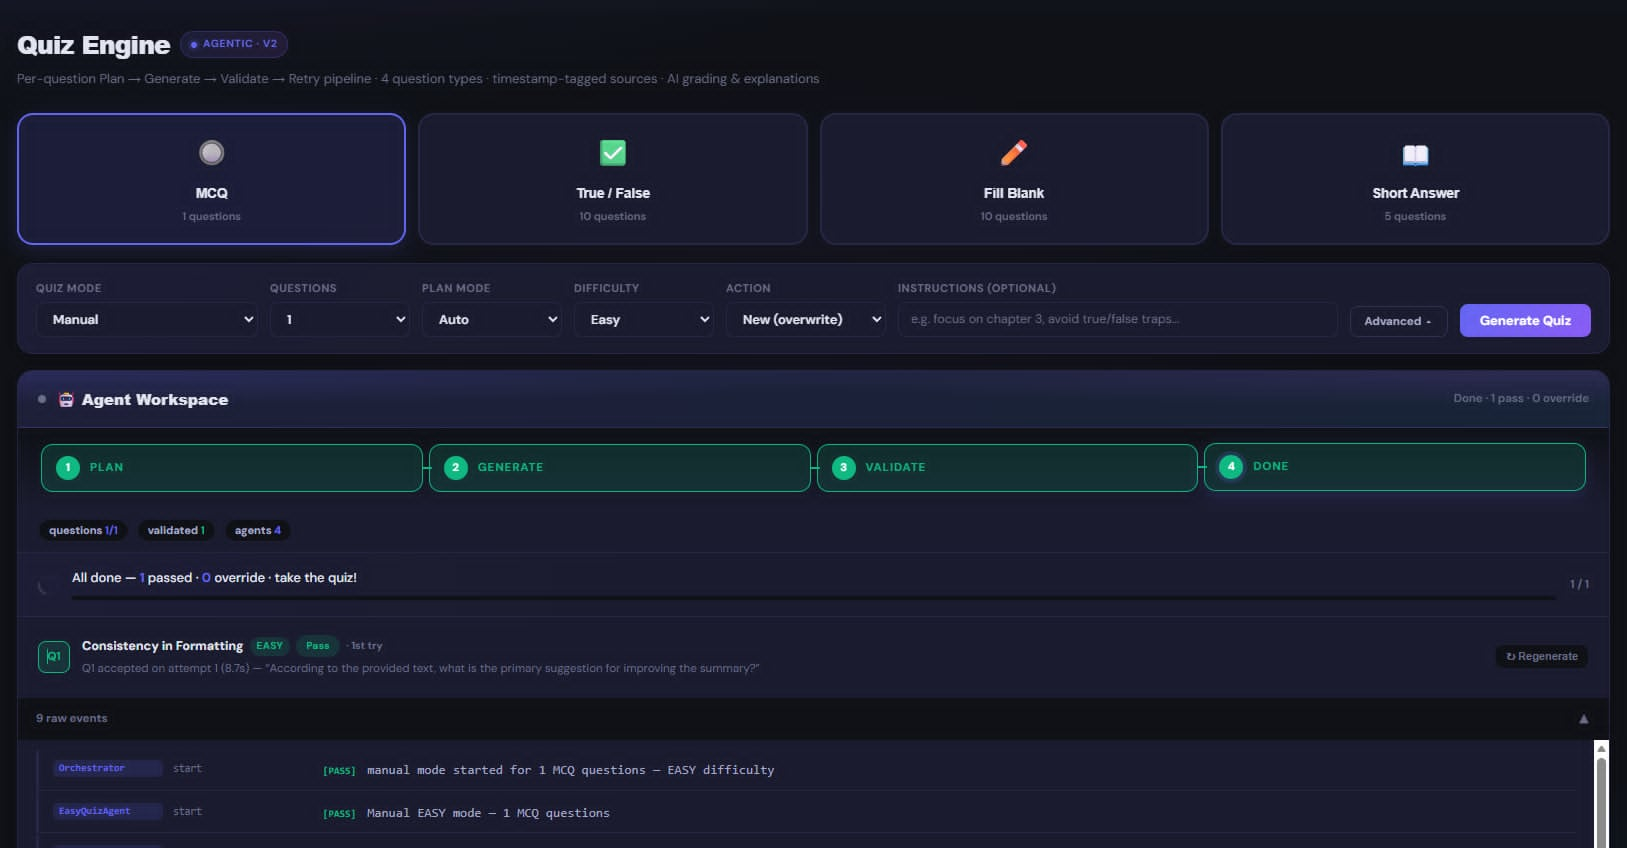
\includegraphics[width=\linewidth]{ui.jpg}
\caption{The Quiz Engine and its live Agent Workspace. The four stage indicators
across the top track the pipeline in real time as it runs. Beneath them, the counters
report questions completed, questions validated and agents active, and each generated
question appears as its own row recording the topic, the target difficulty, the
verdict, the attempt on which it was accepted and the time taken. The row shown here
was accepted on the first attempt in $8.7$ seconds. The raw event log at the bottom
names the agent responsible for every step, so a run can be audited after the fact
rather than inferred from its output.}
\label{fig:ui-workspace}
\end{figure}

\begin{figure}[H]
\centering
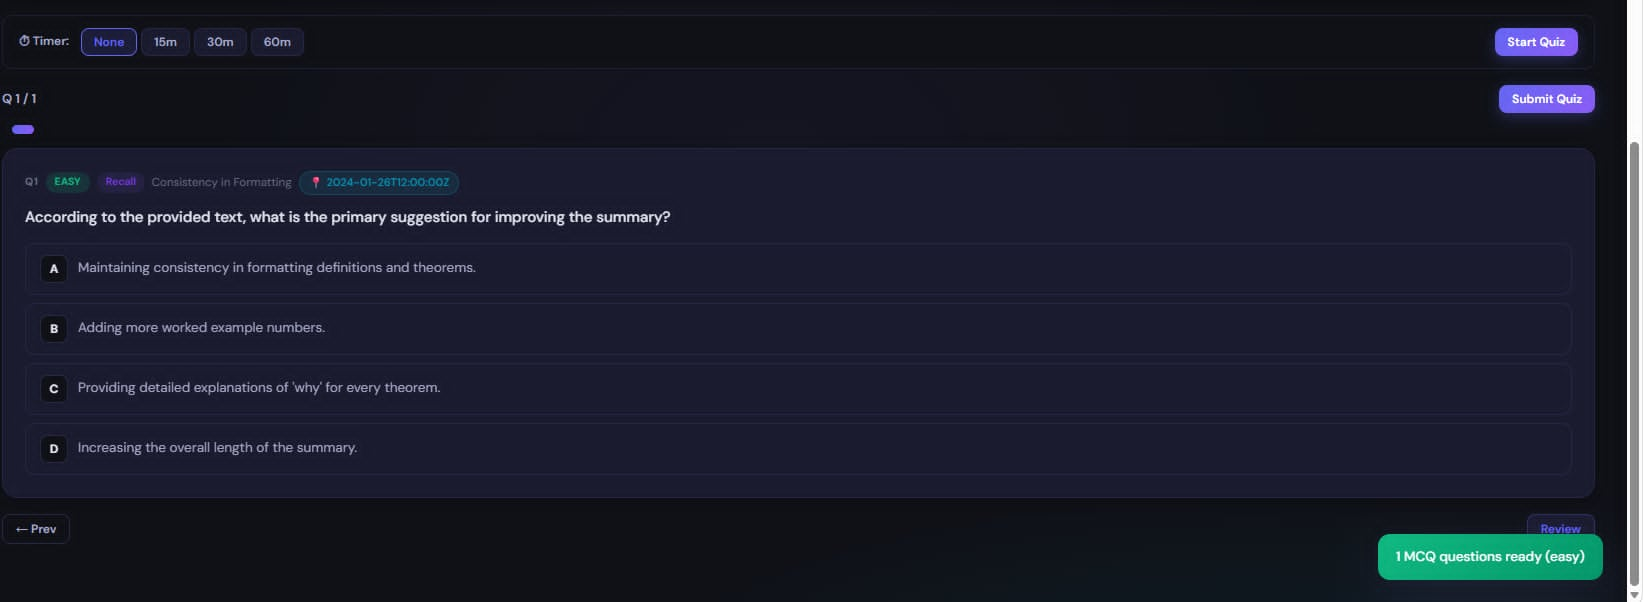
\includegraphics[width=\linewidth]{ui2.jpg}
\caption{The quiz-taking view. Each item carries its target difficulty, its Bloom
level and the topic it was planned against, together with the source timestamp of
the lecture material it was grounded in. That timestamp is what allows a student who
doubts an answer to return to the exact moment in the lecture the question came
from, which is the practical safeguard against the failure mode discussed in
Chapter~\ref{ch:impacts}.}
\label{fig:ui-quiz}
\end{figure}

\begin{figure}[H]
\centering
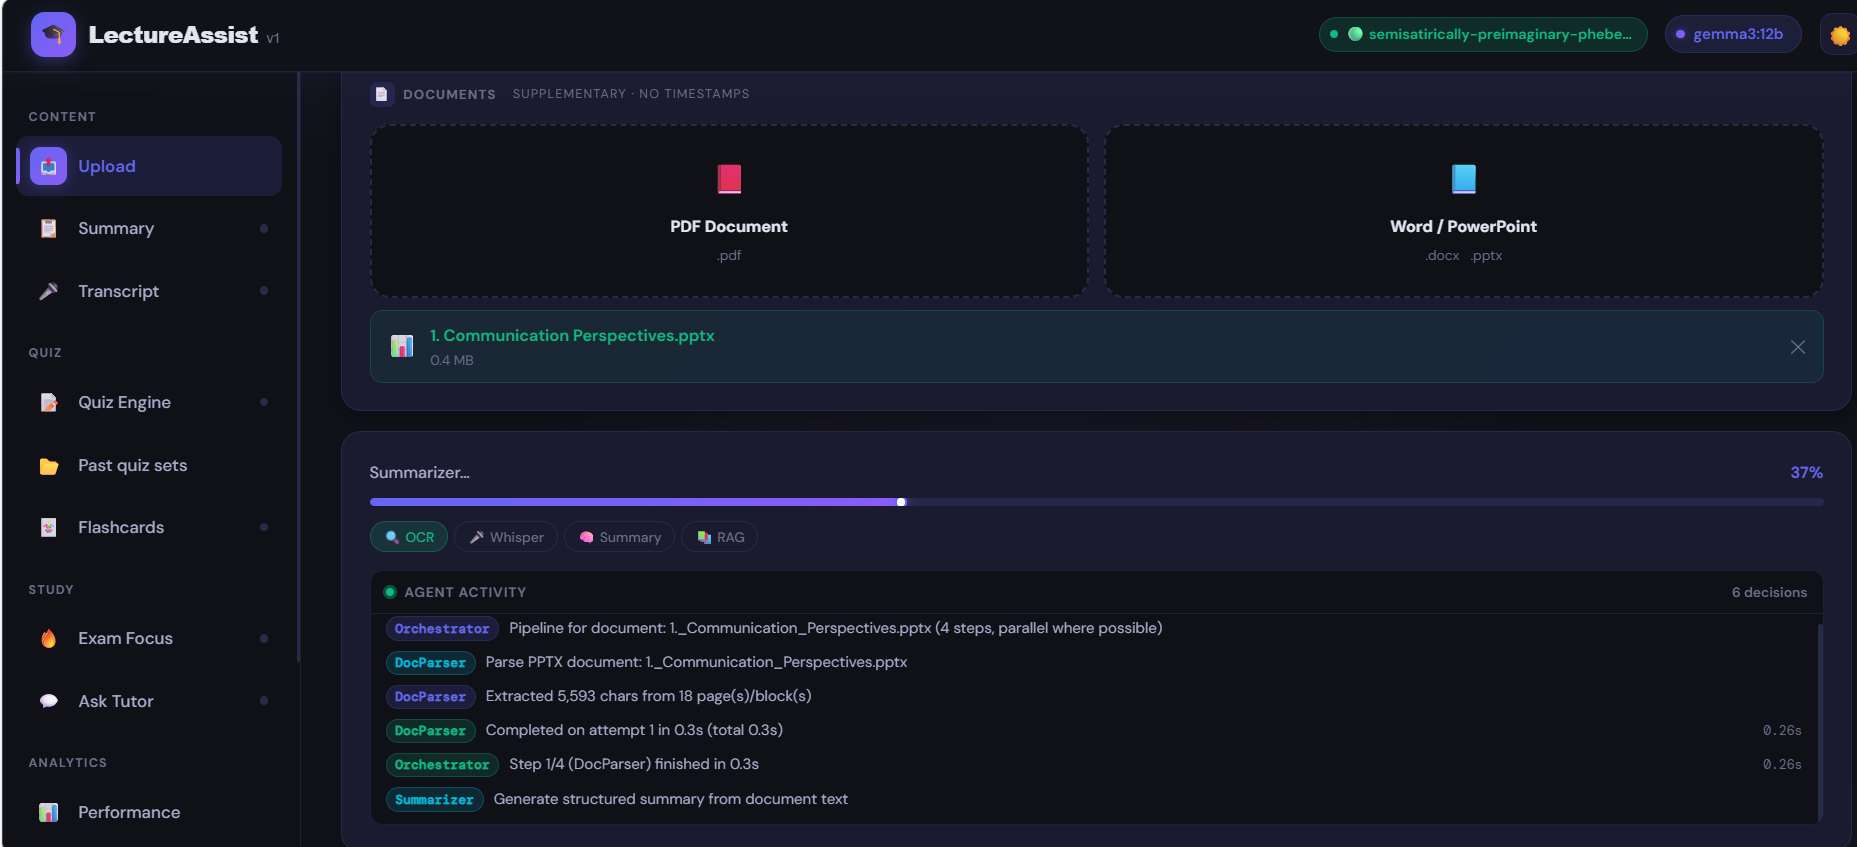
\includegraphics[width=\linewidth]{ui-upload-live.png}
\caption{Processing in progress. The agent activity feed streams each orchestrator
decision as it is taken rather than reporting them only once the run has finished:
the capture shows six decisions logged at $37\%$ completion, with the DocParser
having extracted $5{,}593$ characters from $18$ blocks in $0.3$ seconds and the
Summarizer already started. The stage pills above it track which of OCR, Whisper,
Summary and RAG is currently active.}
\label{fig:ui-live}
\end{figure}

\begin{figure}[H]
\centering
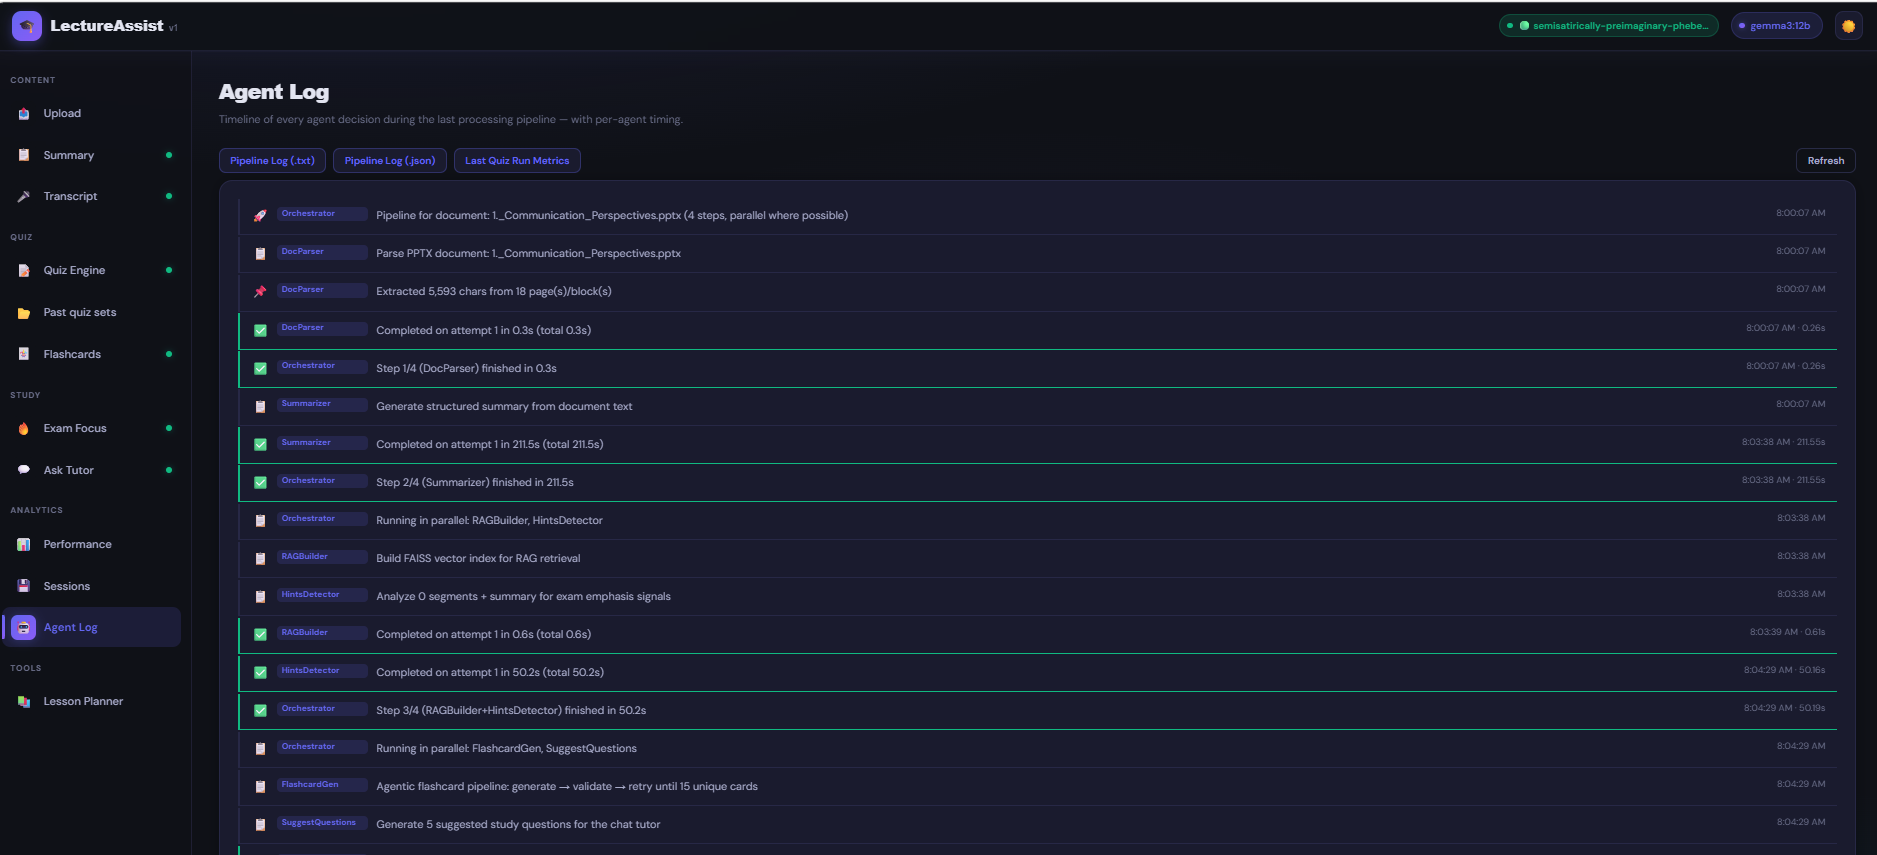
\includegraphics[width=\linewidth]{ui-agentlog.png}
\caption{The agent log for a completed document run, with per-agent timing. The
trail records not only which agent acted but how long each took and which steps the
orchestrator chose to run concurrently: DocParser completed in $0.3$s, the
Summarizer in $211.5$s, and RAGBuilder and HintsDetector were dispatched in parallel,
finishing in $0.6$s and $50.2$s respectively. The pipeline is therefore auditable
after the fact, which is what makes the timing claims in this chapter checkable
rather than asserted.}
\label{fig:ui-agentlog}
\end{figure}

\begin{figure}[H]
\centering
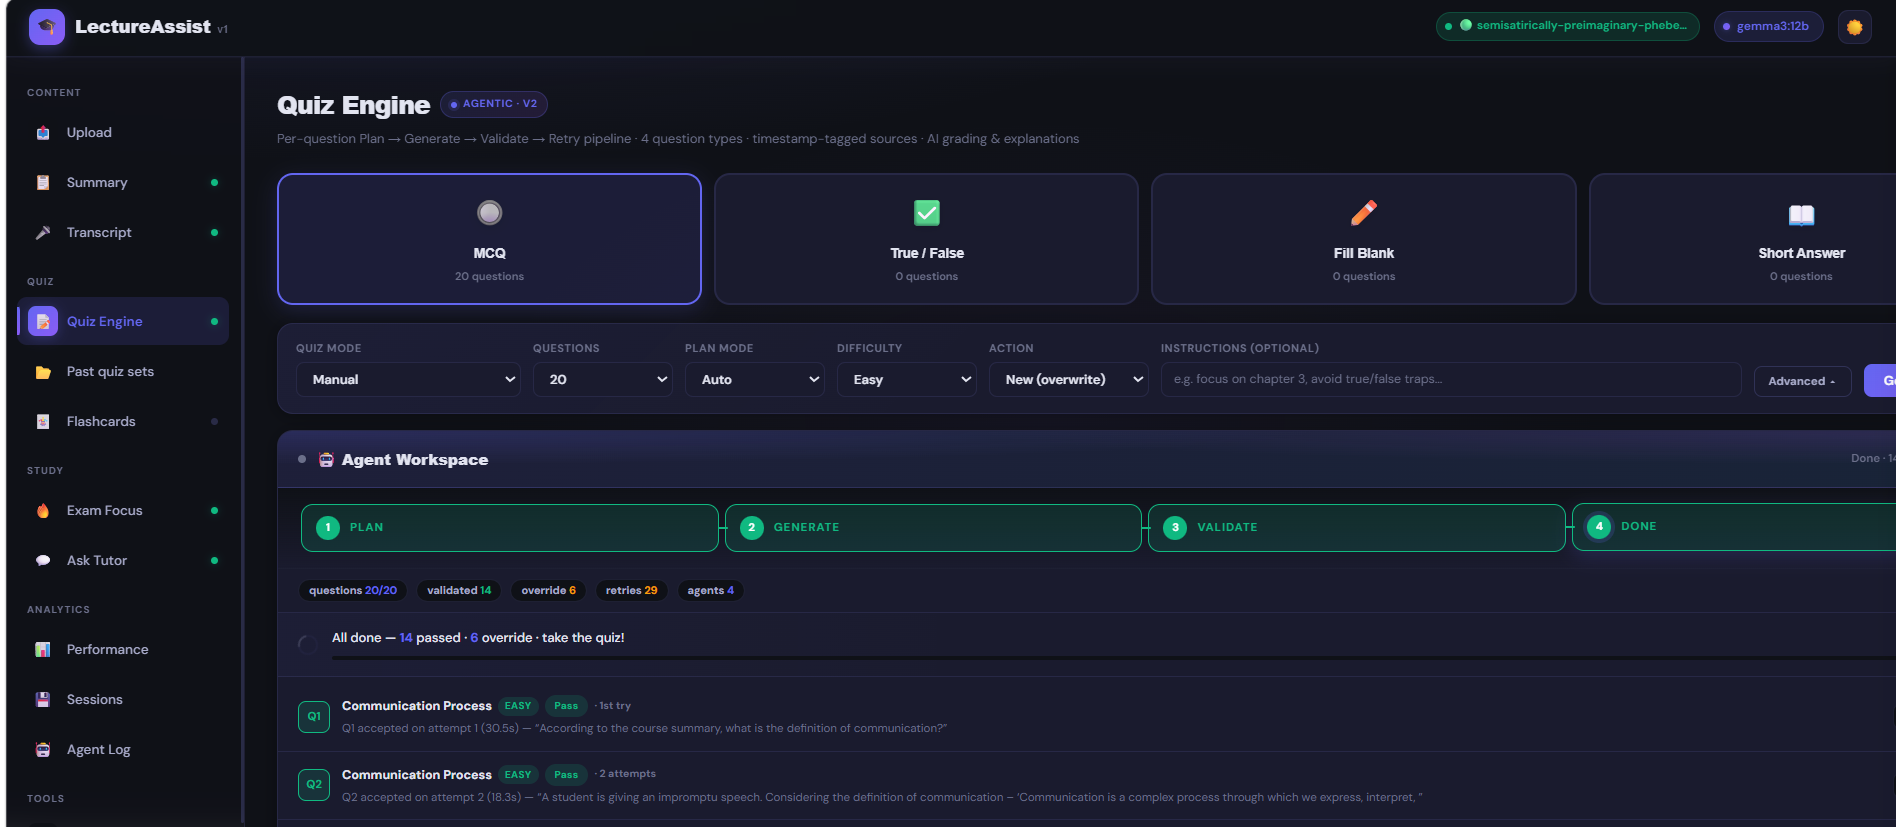
\includegraphics[width=\linewidth]{ui-quiz-run.png}
\caption{A full twenty-question generation. The counters read
\emph{questions $20/20$, validated $14$, override $6$, retries $29$, agents $4$},
and the status line states plainly that $14$ passed and $6$ were kept as overrides.
Twenty accepted questions therefore cost twenty-nine retries, which is the compute
multiplication discussed in Section~\ref{sec:impacts-economic} made visible.}
\label{fig:ui-quizrun}
\end{figure}

\begin{figure}[H]
\centering

\includegraphics[width=\linewidth]{ui-graded.png}
\caption{The graded review, with the source panel open. Each item shows the marked
answer against the student's, the explanation drawn from the retrieved material, and
the lecture timestamp the question was grounded in; selecting that timestamp opens
the source at that moment. Items answered incorrectly are separated from those
answered correctly, so the review surface is also the input to the per-topic
weakness profile of Section~\ref{sec:meth-grading}.}
\label{fig:ui-graded}
\end{figure}

The counters in Figures~\ref{fig:ui-workspace} and~\ref{fig:ui-quizrun} distinguish
questions that passed validation from those kept as overrides, and
Figure~\ref{fig:ui-quizrun} is the more informative of the two because it is a run
in which overrides actually occurred: six of its twenty items exhausted the retry
budget. This distinction is shown rather than hidden for the reason given in
Section~\ref{sec:meth-agentic}: a pipeline that silently recorded an exhausted retry
budget as a clean pass would report an acceptance rate that was a fiction, and the
interface is built to make that impossible. The same figure is also the honest
counterweight to the loop's benefits, since it shows what the loop costs.

\subsection{Multi-tier grading and adaptation}
\label{sec:meth-grading}

Student answers are graded by a cascade chosen to match the question type. MCQ and
True/False are graded by exact key match. Fill-in-the-Blank is graded by a fallback
chain of exact match, then containment, then fuzzy string similarity above a $0.80$
threshold, so that a correct answer is not marked wrong over a typo or a plural.
Short Answer, where no string comparison is adequate, is graded by the $12$B model
against a rubric, which also returns concept-level feedback naming what the student
missed rather than merely marking it incorrect.

Every graded response updates a persistent per-topic profile. The Adaptive Quiz
agent reads that profile and biases the next quiz's topic and difficulty allocation
toward the topics where the student's accuracy is lowest, so that practice
concentrates where it is needed instead of being uniformly distributed.
